% Created 2016-01-08 Fri 16:46
\documentclass[bigger]{beamer}
\usepackage[utf8]{inputenc}
\usepackage[T1]{fontenc}
\usepackage{fixltx2e}
\usepackage{graphicx}
\usepackage{grffile}
\usepackage{longtable}
\usepackage{wrapfig}
\usepackage{rotating}
\usepackage[normalem]{ulem}
\usepackage{amsmath}
\usepackage{textcomp}
\usepackage{amssymb}
\usepackage{capt-of}
\usepackage{hyperref}
\usepackage{minted}
\usepackage{inconsolata}
\usepackage{tikz}
\usepgflibrary{shapes.geometric}
\usetikzlibrary{calc}
\usetikzlibrary{positioning}
\usetikzlibrary{plotmarks}
\usepackage{pgfplots}
\mode<beamer>{\usetheme{EPCC}}
\institute{EPCC, The University of Edinburgh}
\AtBeginSection[]{\begin{frame}\tableofcontents[currentsection]\end{frame}}
\usetheme{default}
\author{Lawrence Mitchell}
\date{Tuesday 22nd January 2013}
\title{Fast, portable unstructured mesh programs}
\hypersetup{
 pdfauthor={Lawrence Mitchell},
 pdftitle={Fast, portable unstructured mesh programs},
 pdfkeywords={},
 pdfsubject={},
 pdfcreator={Emacs 24.5.1 (Org mode 8.3.2)}, 
 pdflang={English}}
\begin{document}

\begin{frame}
\maketitle
\end{frame}


\section{Introduction}
\label{sec:orgheadline3}


\begin{frame}[label={sec:orgheadline1}]{Big picture}
\begin{itemize}
\item lots of computational science solves PDEs
\item in some (arbitrary shape) physical domain
\item applications in
\begin{itemize}
\item ocean dynamics
\item atmospheric dynamics
\item race-car, airplane, building design
\item bone modelling
\item EM signal propagation
\item \ldots{}
\end{itemize}
\end{itemize}
\end{frame}

\begin{frame}[label={sec:orgheadline2}]{Current status quo}
\begin{itemize}
\item Existing software has numerics intimately tied to implementation
\item domain scientist must be expert parallel programmer
\item but science is hard, and programming is hard too
\begin{itemize}
\item state of the art methods take a long time to adopt
\end{itemize}
\end{itemize}
\end{frame}

\section{Code generation for high performance}
\label{sec:orgheadline16}

\begin{frame}[label={sec:orgheadline4}]{Generate, don't transform}
\begin{itemize}
\item Writing compilers is hard
\begin{itemize}
\item but writing domain-specific compilers is "easy"
\end{itemize}
\item with the correct abstractions
\begin{itemize}
\item we can generate good code
\item without having to work hard analysing the problem
\end{itemize}
\end{itemize}
\end{frame}

\begin{frame}[label={sec:orgheadline5}]{Make the parallelism explicit}
\begin{itemize}
\item express \emph{what} to do, not \emph{how} to do it
\item can choose best execution strategy
\begin{itemize}
\item different for CPU/GPU
\item different for shared memory/distributed memory
\end{itemize}
\end{itemize}
\end{frame}

\begin{frame}[fragile,label={sec:orgheadline6}]{A typical kernel}
 \begin{minted}[frame=none,xleftmargin=1em,xrightmargin=1em,fontsize=\scriptsize,mathescape]{python}
for element in mesh_elements:
  nodes = mesh_nodes[element]
  some_function(nodes, element)
\end{minted}
\begin{itemize}
\item loop over elements
\item access nodes related to element and do some computation
\end{itemize}
\end{frame}

\begin{frame}[fragile,label={sec:orgheadline7}]{Parallelising things}
 \begin{itemize}
\item static analysis impossible
\begin{itemize}
\item map from elements to node runtime-only
\end{itemize}
\item By hand, colour dependency graph
\end{itemize}
\begin{minted}[frame=none,xleftmargin=1em,xrightmargin=1em,fontsize=\scriptsize,mathescape]{python}
for col in mesh_colors:
  # do in (shared memory) parallel
  for element in mesh_elements[col]:
    nodes = mesh_nodes[element]
    some_function(nodes, element)
\end{minted}
\end{frame}

\begin{frame}[label={sec:orgheadline8}]{But what if we have a new platform}
\begin{itemize}
\item On GPUs need to
\begin{itemize}
\item manually manage shared memory
\item employ two-level colouring (both thread blocks and threads)
\end{itemize}
\item And then we get time on a non-GPU system
\end{itemize}
\end{frame}

\begin{frame}[label={sec:orgheadline9}]{The Moon, on a stick}
\begin{itemize}
\item We want:
\begin{itemize}
\item easy programmability
\item platform-portability (CPU/GPU/MIC, \ldots{})
\item performance across platforms
\end{itemize}
\end{itemize}
\end{frame}

\begin{frame}[label={sec:orgheadline10}]{A solution}
\begin{itemize}
\item User writes numerical kernel
\begin{itemize}
\item expresses iteration over mesh
\item accessing data, with access descriptors
\end{itemize}
\item runtime library
\begin{itemize}
\item analyses iteration for parallelism
\item generates code to execute kernel
\end{itemize}
\end{itemize}
\end{frame}

\begin{frame}[label={sec:orgheadline11}]{PyOP2}
\begin{itemize}
\item A library for unstructured mesh computations
\begin{itemize}
\item \url{http://github.com/OP2/PyOP2}
\end{itemize}
\item Implements the OP2 abstraction (\url{http://www.oerc.ox.ac.uk/research/op2})
\item data types
\begin{description}
\item[{\emph{Set}}] e.g. Nodes or elements of a mesh
\item[{\emph{Dat}}] data defined on a Set (one entry per set element)
\item[{\emph{Map}}] a mapping between two sets (e.g. elements to nodes)
\item[{\emph{Global}}] global data (one entry)
\item[{\emph{Kernel}}] a piece of code to execute over the mesh
\end{description}
\end{itemize}
\end{frame}

\begin{frame}[fragile,label={sec:orgheadline12}]{PyOP2 continued}
 \begin{itemize}
\item access descriptors
\begin{itemize}
\item READ, RW, WRITE, INC
\end{itemize}
\item iteration construct
\begin{description}
\item[\verb~par\_loop~] execute a Kernel over every element in a \texttt{Set}
\end{description}
\end{itemize}
\end{frame}

\begin{frame}[fragile,label={sec:orgheadline13}]{An example}
 \begin{minted}[frame=none,xleftmargin=1em,xrightmargin=1em,fontsize=\scriptsize,mathescape]{python}
par_loop(kernel, elements,
         element_data(IdentityMap, READ),
         node_data(elem_node, WRITE),
         elem_count(INC))
\end{minted}

\begin{itemize}
\item executes \emph{kernel} for each ele in elements
\begin{description}
\item[{first argument}] data corresponding to ele (read-only)
\item[{second argument}] the nodes of this ele (written)
\item[{third argument}] a global counter (incremented)
\end{description}

\item runtime knows it has to care about data dependencies for
\begin{itemize}
\item write to \verb~node_data~
\item increment into \verb~elem_count~
\end{itemize}
\end{itemize}
\end{frame}

\begin{frame}[label={sec:orgheadline14}]{What goes on under the hood?}
\begin{itemize}
\item kernel is a piece of C code (user provided)
\begin{itemize}
\item conforms to an API
\end{itemize}
\item PyOP2 runtime \emph{generates} code
\item different parallel targets
\begin{itemize}
\item Serial CPU (partly for verification)
\item CUDA
\item OpenCL
\item OpenMP
\end{itemize}
\item MPI for distributed memory (as of last weekend)
\item switching from CPU to GPU needs
\begin{itemize}
\item one line change in source code
\end{itemize}
\end{itemize}
\end{frame}

\begin{frame}[label={sec:orgheadline15}]{A picture}
\begin{center}
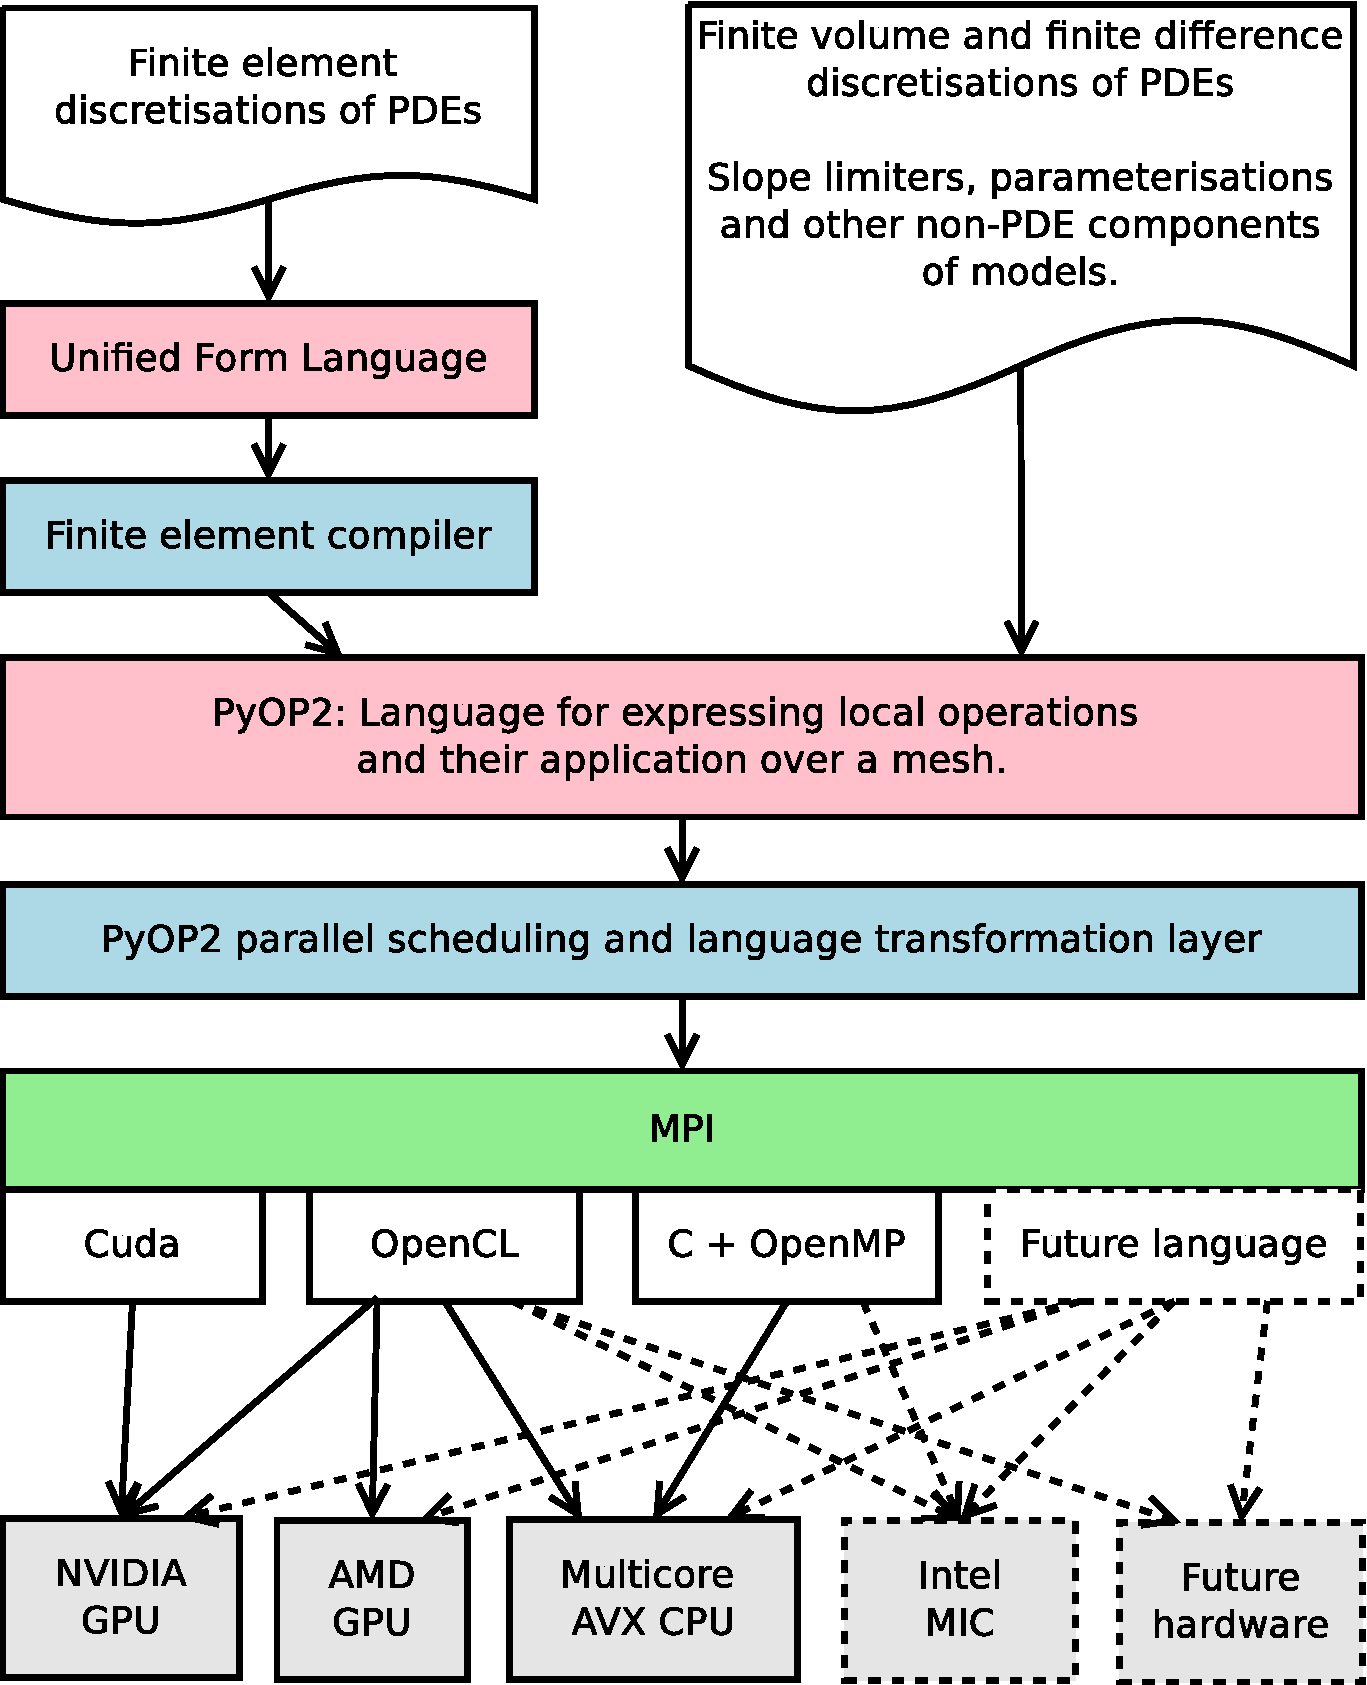
\includegraphics[height=.9\textheight]{01-22-HIPEAC-PyOP2.figures/abstractions.pdf}
\end{center}
\end{frame}

\section{More automation}
\label{sec:orgheadline21}
\begin{frame}[label={sec:orgheadline17}]{flop.py}
\begin{itemize}
\item a high-performance implementation of UFL
\begin{itemize}
\item The Unified Form Language (\url{https://launchpad.net/UFL})
\end{itemize}
\item Uses Fluidity as the mesh framework
\begin{itemize}
\item (\url{http://launchpad.net/fluidity})
\end{itemize}
\item express weak form of PDE
\begin{itemize}
\item automatically generate the "user" kernel
\item and its execution over the mesh
\end{itemize}
\end{itemize}
\end{frame}

\begin{frame}[fragile,label={sec:orgheadline18}]{An example}
 \begin{itemize}
\item Helmholtz equation (the easy one)
\end{itemize}
\begin{displaymath}
-\nabla^2 u + \eta u = f \;\; \eta > 0
\end{displaymath}
\begin{itemize}
\item weak form (suitable BCs)
\end{itemize}
\begin{displaymath}
\int_x (\nabla u \cdot \nabla v - \eta u v) dx = \int_x v f dx
\end{displaymath}
\begin{itemize}
\item UFL
\end{itemize}
\begin{minted}[frame=none,xleftmargin=1em,xrightmargin=1em,fontsize=\scriptsize,mathescape]{python}
f = state.scalar_fields["Tracer"]
v = TestFunction(f)
u = TrialFunction(f)
a = (inner(grad(u), grad(v)) - eta * u * v)*dx
L = v * f * dx
solve(a == L, f)
\end{minted}
\end{frame}

\begin{frame}[label={sec:orgheadline19}]{A picture}
\begin{center}
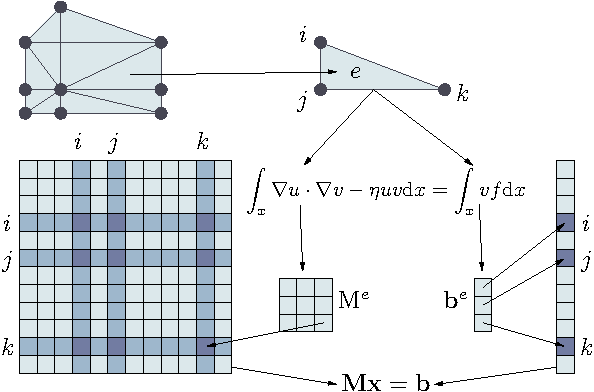
\includegraphics[width=.9\linewidth]{01-22-HIPEAC-PyOP2.figures/assembly-crop.pdf}
\end{center}
\end{frame}

\begin{frame}[label={sec:orgheadline20}]{What happens under the hood}
\begin{itemize}
\item Generate local element assembly kernel
\begin{itemize}
\item C code
\end{itemize}
\item express execution over mesh in PyOP2
\begin{itemize}
\item global assembly of system
\begin{itemize}
\item can swap out different strategies, depending on hardware
\end{itemize}
\end{itemize}
\item solve it
\begin{itemize}
\item using linear algebra libraries
\item PETSc on CPU
\item Currently CUSP in CUDA
\end{itemize}
\end{itemize}
\end{frame}

\section{Performance numbers}
\label{sec:orgheadline26}

\begin{frame}[label={sec:orgheadline22}]{Was it worth it?}
\begin{itemize}
\item DOLFIN (\url{http://launchpad.net/dolfin}) already implements UFL
\begin{itemize}
\item why bother?
\end{itemize}
\item We're faster
\end{itemize}
\begin{center}
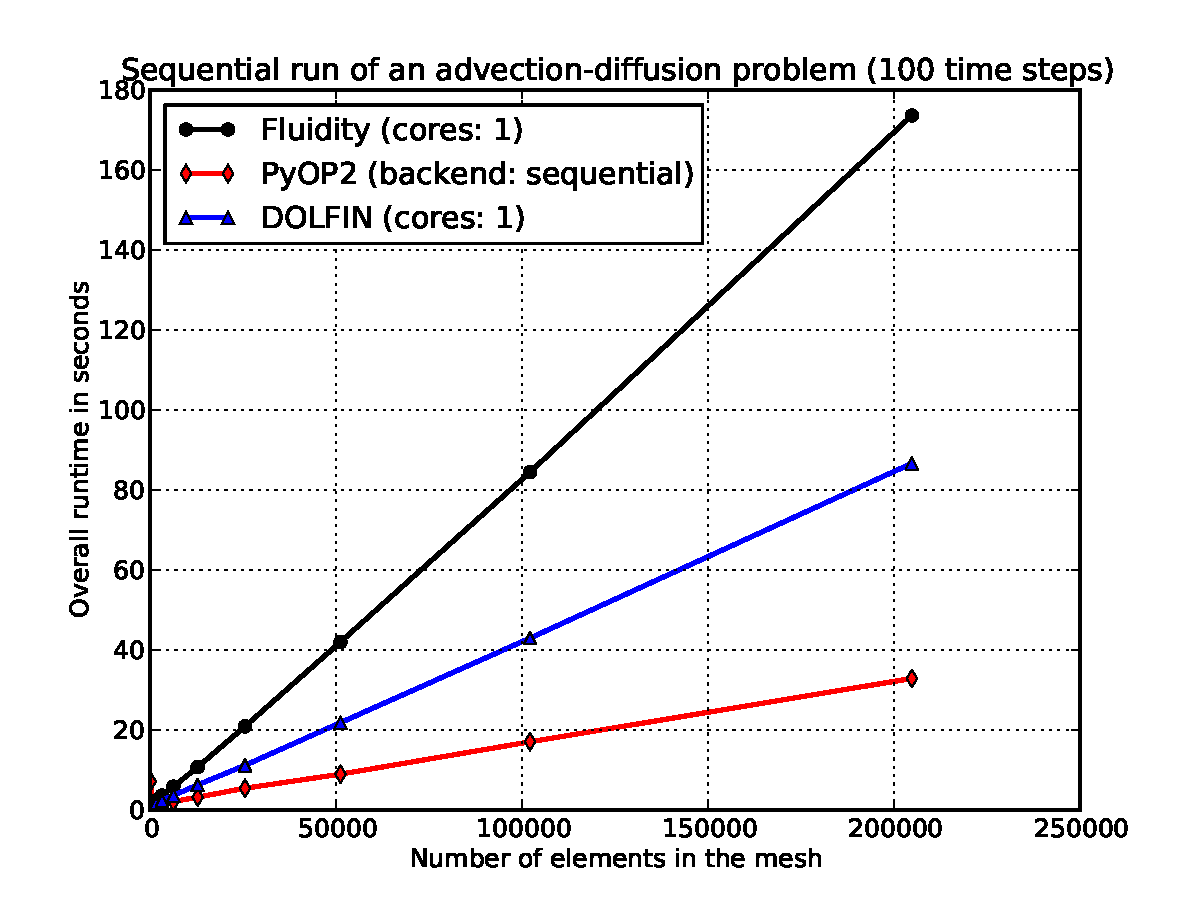
\includegraphics[width=.75\textheight]{01-22-HIPEAC-PyOP2.figures/sequential.pdf}
\end{center}
\end{frame}

\begin{frame}[label={sec:orgheadline23}]{Also, you get GPUs}
\begin{center}
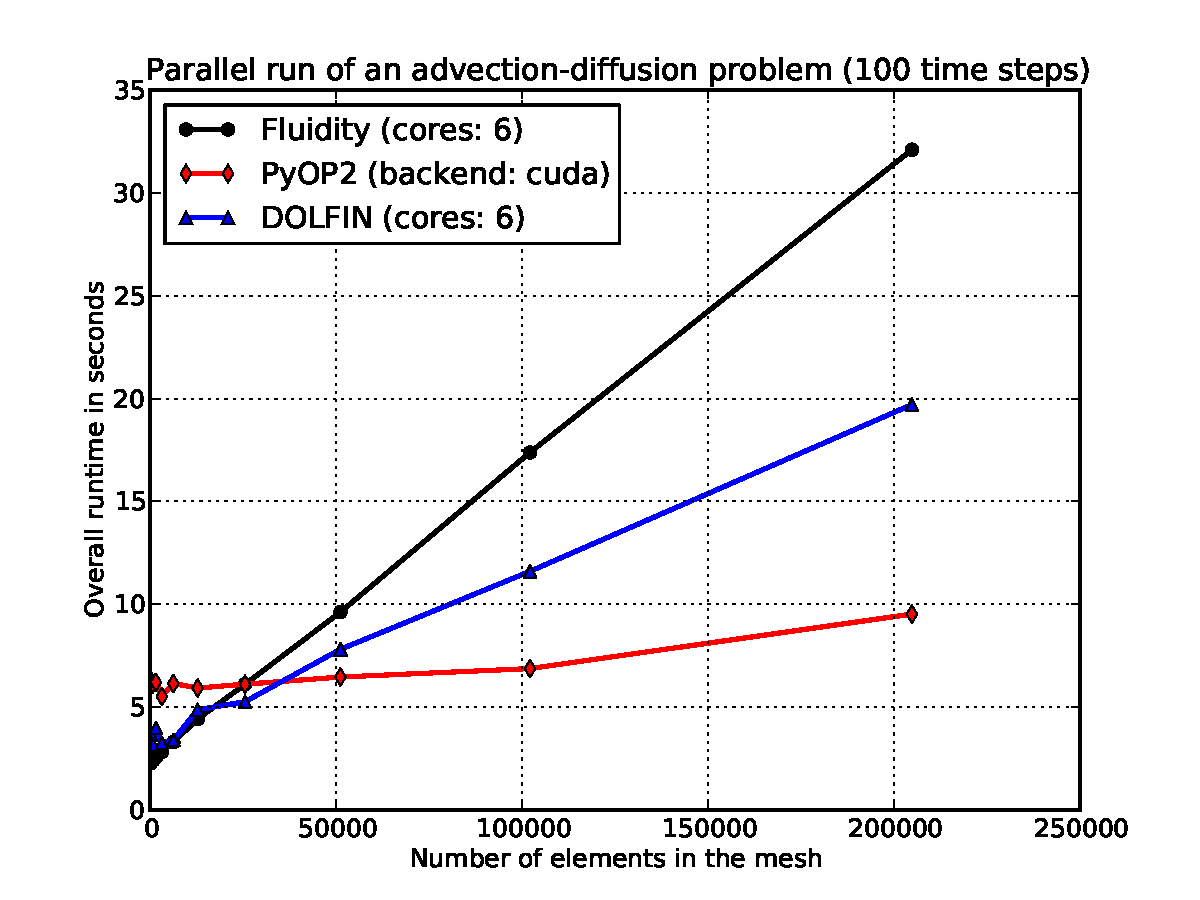
\includegraphics[width=.9\textheight]{01-22-HIPEAC-PyOP2.figures/cuda.pdf}
\end{center}
\end{frame}

\begin{frame}[label={sec:orgheadline24}]{What can you do now?}
\begin{itemize}
\item CG-like discretisations
\item Strong BCs
\item Weak BCs
\end{itemize}
\end{frame}

\begin{frame}[label={sec:orgheadline25}]{What's coming soon?}
\begin{itemize}
\item DG-like discretisations (end of January)
\begin{itemize}
\item all the bits are there, but untested, therefore broken
\end{itemize}
\item MPI-parallel (February)
\begin{itemize}
\item seemingly working as of this weekend
\end{itemize}
\item Mixed function spaces (February)
\begin{itemize}
\item allow Physics-based preconditioning
\end{itemize}
\item The rest of UFL (March, hopefully)
\end{itemize}
\end{frame}

\section{And finally}
\label{sec:orgheadline29}

\begin{frame}[label={sec:orgheadline27}]{Thanks}
\begin{itemize}
\item PyOP2 development is funded in part by MAPDES (EP/I00677X/1, EP/I006079/1)
\begin{description}
\item[{Imperial}] David Ham, Paul Kelly, Nicolas
Loriant, Graham Markall, Florian Rathgeber
\item[{Oxford}] Mike Giles, Gihan Mudalige, Istvan Reguly
\end{description}
\item And APOS-EU (FP7/277481)
\begin{description}
\item[{EPCC}] Me
\end{description}
\end{itemize}
\end{frame}

\begin{frame}[label={sec:orgheadline28}]{Questions?}
\begin{itemize}
\item comments?
\item anything else?
\end{itemize}
\end{frame}
\end{document}
